\documentclass[10pt]{beamer}

% Packages
\usepackage[utf8]{inputenc}
\usepackage[T1]{fontenc}
\usepackage{amsmath, amssymb, amsthm}
\usepackage{graphicx}
\usepackage{booktabs}
\usepackage{hyperref}
\usepackage{tikz}
\usetikzlibrary{shapes,arrows,positioning}

% Theme settings
\usetheme{default}
\usecolortheme{default}
\usefonttheme{professionalfonts}

\definecolor{ImperialBlue}{RGB}{0, 62, 116}
\definecolor{DarkGray}{RGB}{51, 51, 51}
\definecolor{LightGray}{RGB}{245, 245, 245}
\definecolor{AccentOrange}{RGB}{214, 96, 77}
\definecolor{AccentGreen}{RGB}{46, 139, 87}

% Apply colors
\setbeamercolor{frametitle}{fg=ImperialBlue, bg=white}
\setbeamercolor{title}{fg=ImperialBlue}
\setbeamercolor{structure}{fg=ImperialBlue}
\setbeamercolor{normal text}{fg=DarkGray}
\setbeamercolor{block title}{fg=white, bg=ImperialBlue}
\setbeamercolor{block body}{fg=DarkGray, bg=LightGray}
\setbeamercolor{itemize item}{fg=ImperialBlue}
\setbeamercolor{enumerate item}{fg=ImperialBlue}

% Remove navigation symbols
\setbeamertemplate{navigation symbols}{}

% Customize frame title
\setbeamertemplate{frametitle}{
  \vspace{0.5em}
  \insertframetitle
  \vspace{0.3em}
}

% Customize itemize
\setbeamertemplate{itemize items}[circle]
\setlength{\leftmargini}{1.5em}

% Footer
\setbeamertemplate{footline}{
  \leavevmode%
  \hbox{%
  \begin{beamercolorbox}[wd=.333333\paperwidth,ht=2.25ex,dp=1ex,left]{author in head/foot}%
    \hspace{1em}\usebeamerfont{author in head/foot}\insertshortauthor
  \end{beamercolorbox}%
  \begin{beamercolorbox}[wd=.333333\paperwidth,ht=2.25ex,dp=1ex,center]{title in head/foot}%
    \usebeamerfont{title in head/foot}\insertshorttitle
  \end{beamercolorbox}%
  \begin{beamercolorbox}[wd=.333333\paperwidth,ht=2.25ex,dp=1ex,right]{date in head/foot}%
    \usebeamerfont{date in head/foot}\insertshortdate{}\hspace*{2em}
    \insertframenumber{} / \inserttotalframenumber\hspace*{2ex} 
  \end{beamercolorbox}}%
  \vskip0pt%
}

% Title page customization
\setbeamertemplate{title page}{
  \vbox{}
  \vfill
  \begingroup
    \centering
    {\usebeamercolor[fg]{title}\usebeamerfont{title}\inserttitle\par}
    \vskip0.5em
    {\usebeamercolor[fg]{subtitle}\usebeamerfont{subtitle}\insertsubtitle\par}
    \vskip2em
    {\usebeamercolor[fg]{author}\usebeamerfont{author}\insertauthor\par}
    \vskip0.5em
    {\usebeamercolor[fg]{institute}\usebeamerfont{institute}\insertinstitute\par}
    \vskip1em
    {\usebeamercolor[fg]{date}\usebeamerfont{date}\insertdate\par}
  \endgroup
  \vfill
}

% Commands for highlighting
\newcommand{\emphbox}[1]{\colorbox{LightGray}{\textcolor{DarkGray}{#1}}}
\newcommand{\highlight}[1]{\textcolor{AccentOrange}{\textbf{#1}}}
\newcommand{\good}[1]{\textcolor{AccentGreen}{#1}}
\newcommand{\bad}[1]{\textcolor{AccentOrange}{#1}}

%----------------------------------------------------------------------------------------
\title{Blockchain Economics}
\subtitle{ECOM215: Blockchain Economics and Digital Assets}
\author{Dr Daniele Bianchi}
\institute{Queen Mary, University of London}
\date{Semester B, 2025/2026}
%----------------------------------------------------------------------------------------

\begin{document}

\AtBeginSection[]{
  \begin{frame}[plain]
    \vfill
    \begin{center}
      {\Large\color{ImperialBlue}\insertsection}
    \end{center}
    \vfill
  \end{frame}
}

\begin{frame}[plain]
  \titlepage
\end{frame}

\begin{frame}{Today's Agenda}
  \tableofcontents
\end{frame}

%----------------------------------------------------------------------------------------
\section{The Consensus Problem}
%----------------------------------------------------------------------------------------

\begin{frame}{Why Consensus Matters}
  Recall from Topic 1: blockchain is a shared ledger with no central authority.
  
  \vspace{1em}
  \textbf{The fundamental question:}
  \begin{center}
    \large How do strangers agree on the state of a shared database\\when some of them might be lying?
  \end{center}
  
  \vspace{1em}
  This is the \highlight{consensus problem}---and solving it is what makes blockchain work.
  
  \vspace{1em}
  \textbf{What we need:}
  \begin{itemize}
    \item All honest participants agree on the same transaction history
    \item Dishonest participants cannot corrupt the ledger
    \item The system keeps working even if some nodes fail or misbehave
  \end{itemize}
\end{frame}

\begin{frame}{The Double-Spend Problem}
  \textbf{Digital cash has a unique problem}: data can be copied perfectly.
  
  \vspace{1em}
  \textbf{Example:}
  \begin{enumerate}
    \item Alice has 1 BTC
    \item Alice sends 1 BTC to Bob (Transaction A)
    \item Alice \textit{simultaneously} sends the same 1 BTC to Carol (Transaction B)
    \item Which transaction is valid?
  \end{enumerate}
  
  \vspace{1em}
  With physical cash, this is impossible---you can't hand the same note to two people.
  
  \vspace{0.5em}
  With digital cash, both transactions are valid copies. \highlight{Someone must decide which one counts.}
  
  \vspace{1em}
  \textbf{Traditional solution}: A bank maintains the authoritative ledger.
  
  \textbf{Blockchain solution}: The network reaches consensus on transaction ordering.
\end{frame}

\begin{frame}{Byzantine Fault Tolerance}
  \begin{block}{The Byzantine Generals Problem}
    How can distributed parties reach agreement when some participants may be unreliable or actively malicious?
  \end{block}
  
  \vspace{0.5em}
  \textbf{The setup}: Generals surrounding a city must coordinate attack or retreat. They can only communicate by messenger. Some generals may be traitors sending conflicting messages.
  
  \vspace{1em}
  \textbf{The blockchain parallel}:
  \begin{itemize}
    \item Thousands of nodes must agree on transaction history
    \item Some nodes might be offline, buggy, or malicious
    \item The system must produce a single consistent ledger anyway
  \end{itemize}
  
  \vspace{1em}
  A blockchain consensus protocol must be \highlight{Byzantine fault tolerant}---it works correctly even when some participants are adversarial.
\end{frame}

\begin{frame}{What Makes Good Consensus?}
  A consensus protocol should deliver:
  \begin{center}
  \begin{tabular}{lp{7.5cm}}
    \toprule
    \textbf{Property} & \textbf{Meaning} \\
    \midrule
    Safety & Honest nodes agree on the same history \\
%    Liveness & Valid transactions eventually get confirmed \\
    Fault tolerance & System works despite failures/attacks \\
    Decentralisation & No single party controls outcomes \\
    Efficiency & Resources aren't wasted unnecessarily \\
    \bottomrule
  \end{tabular}
  \end{center}
  
  \vspace{1em}
  \textbf{The challenge}: These properties often conflict. More security may mean less efficiency. More decentralisation may mean slower consensus.
  
  \vspace{1em}
  This tension is formalised as the \highlight{blockchain trilemma} (later this lecture).
\end{frame}

%----------------------------------------------------------------------------------------
\section{Proof-of-Work}
%----------------------------------------------------------------------------------------

\begin{frame}{The Bitcoin Innovation}
  Before Bitcoin (2009), decentralised digital cash had failed because of the double-spend problem.
  
  \vspace{1em}
  \textbf{Satoshi Nakamoto's insight}: Make adding blocks \textit{computationally expensive}.
  
  \vspace{0.5em}
  \begin{itemize}
    \item Participants (``miners'') compete to solve a cryptographic puzzle
    \item The winner gets to propose the next block and receives a reward (newly minted coins + fees)
    \item Other nodes verify and accept the valid block
  \end{itemize}
  
  \vspace{1em}
  \textbf{Why this works}:
  \begin{itemize}
    \item Attacking the network requires out-computing all honest miners
    \item Cheating is expensive (you spend resources without receiving the reward), whereas honest behaviour is profitable
    \item No central authority decides who adds blocks
  \end{itemize}

  \vspace{0.5em}
  This is \highlight{Proof-of-Work} (PoW): prove you expended computational resources to compete in good faith.
\end{frame}

\begin{frame}{How Mining Works}
\textbf{The puzzle}: Find a random number (``nonce'') that, when hashed with the block data, produces an output starting with a certain number of zeros.\footnote{The protocol sets how many zeros are required, adjusting automatically to keep block production steady (10 minutes for Bitcoin).}
  
  \vspace{0.5em}
  Since hash outputs are unpredictable, there's no shortcut---miners try billions of numbers until one works.
  
  \vspace{1em}
  \textbf{The process}:
  \begin{enumerate}
    \item Collect pending transactions into a candidate block
    \item Try random nonces until one meets the difficulty target
    \item Broadcast the winning block to the network
    \item Other nodes verify (instantly) and append the block to their chain
    \item The winner receives a \highlight{block reward} and \highlight{transaction fees}
  \end{enumerate}

  \vspace{1em}
  \textbf{Key insight}: Finding a valid nonce requires billions of guesses, but verifying one takes a single operation---hash the winner's answer and check whether it meets the target.
\end{frame}

\begin{frame}{Difficulty Target Adjustment}
  Bitcoin targets one block every \highlight{10 minutes} on average.
  
  \vspace{1em}
  \textbf{Problem}: If more miners join, blocks would be found faster.
  
  \textbf{Solution}: The protocol automatically adjusts difficulty every 2,016 blocks ($\approx$ 2 weeks).
  
\begin{figure}
    \centering
    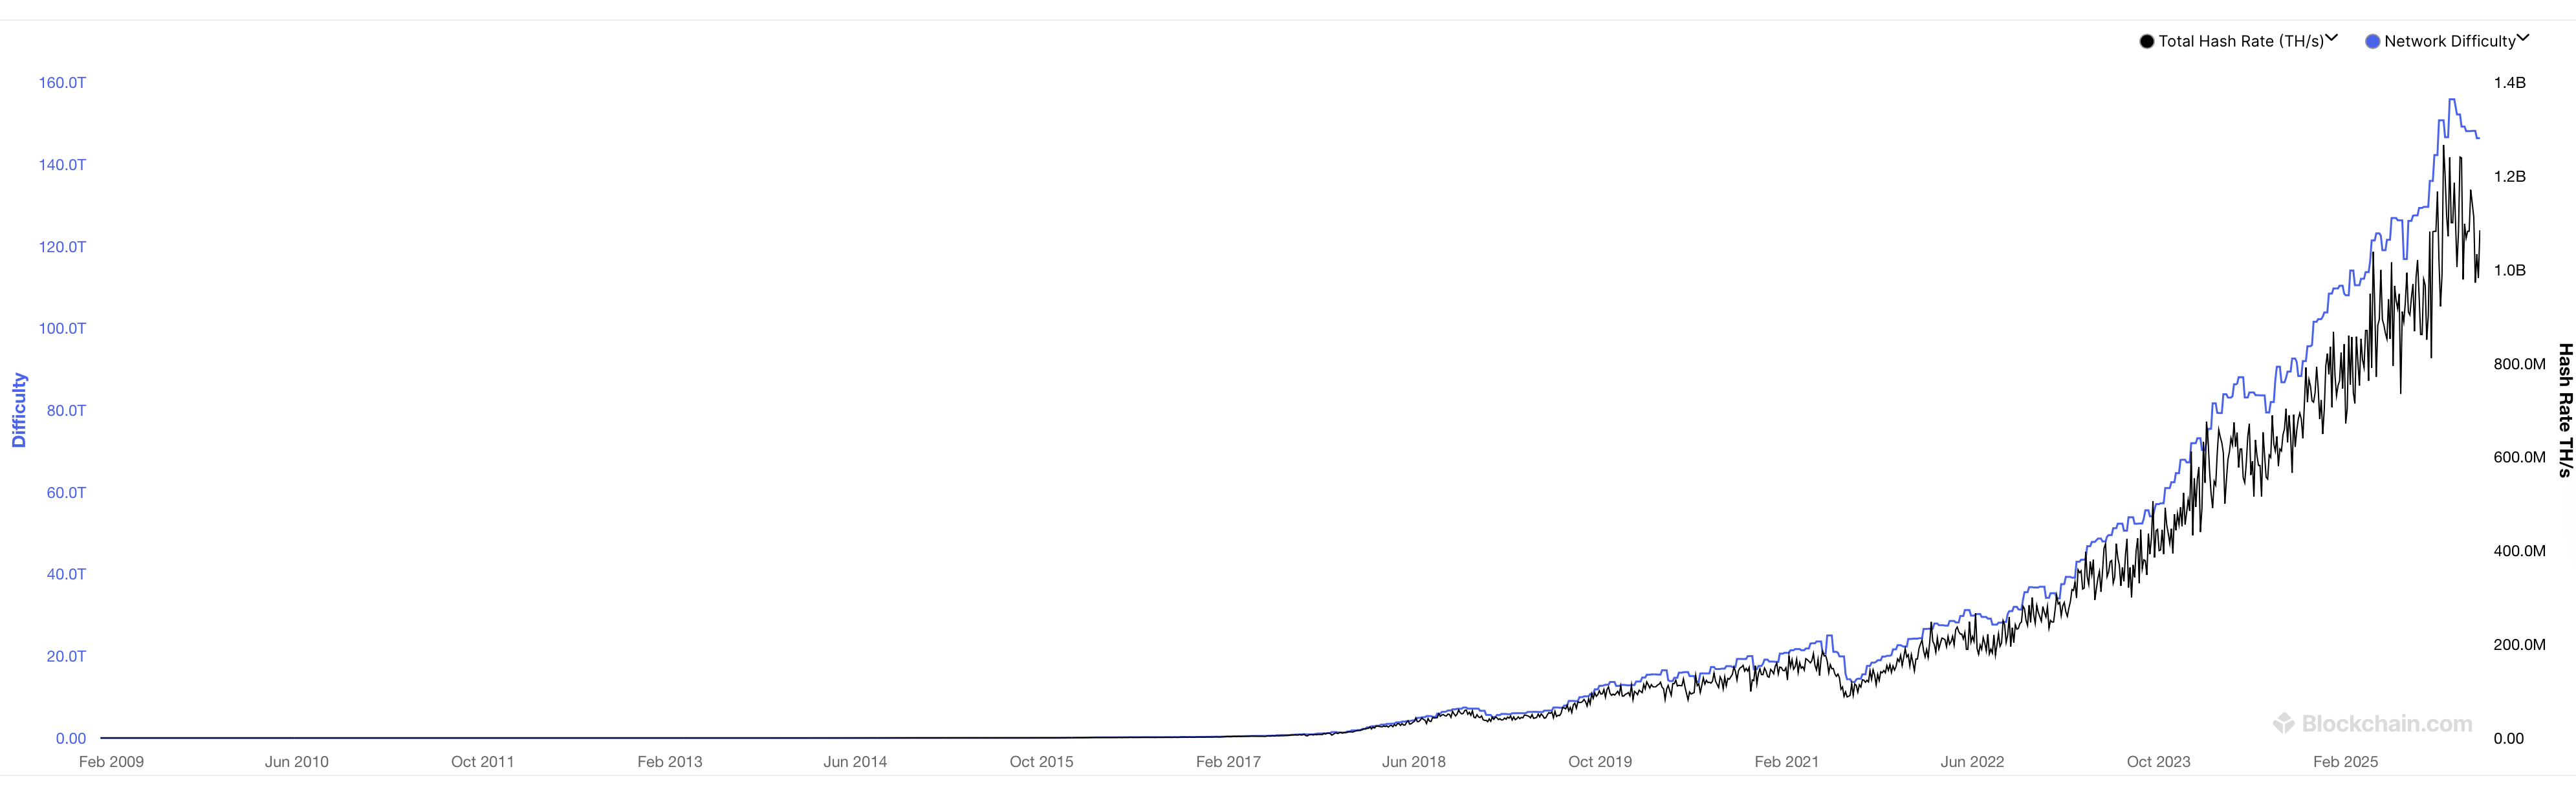
\includegraphics[width=1\linewidth]{Figures/BTC hash vs difficulty.png}
\end{figure}
  
  \textbf{Implication}: Mining is an \highlight{arms race}. More computing power improves your \textit{relative} chance of winning but doesn't increase total block production.
\end{frame}

\begin{frame}{Block Rewards and Halving}
  Miners receive two types of compensation:
  
  \vspace{0.5em}
  \begin{enumerate}
    \item \textbf{Block subsidy}: Newly created bitcoins (currently 3.125 BTC/block)
    \item \textbf{Transaction fees}: Paid by users for inclusion
  \end{enumerate}
  
  \vspace{1em}
  \textbf{The halving}: The block subsidy is cut in half every 210,000 blocks ($\approx$4 years).
  
  \vspace{0.5em}
  \begin{center}
  \begin{tabular}{ccc}
    \toprule
    \textbf{Date} & \textbf{Block Subsidy} & \textbf{Event} \\
    \midrule
    Jan 2009 & 50 BTC & Genesis \\
    Nov 2012 & 25 BTC & 1st halving \\
    Jul 2016 & 12.5 BTC & 2nd halving \\
    May 2020 & 6.25 BTC & 3rd halving \\
    \good{Apr 2024} & \good{3.125 BTC} & \good{4th halving} \\
    ~2028 & 1.5625 BTC & 5th halving (expected) \\
    \bottomrule
  \end{tabular}
  \end{center}
  
  \vspace{0.5em}
  This creates a \highlight{deflationary supply}: maximum 21 million BTC, reached around 2140.
\end{frame}

\begin{frame}{The Transition to Fee-Based Security}
  As block subsidies decline, transaction fees must compensate miners.
  
  \vspace{1em}
  \textbf{The concern}: Will fees alone provide sufficient security incentive?
  
  
  \vspace{1em}
  \textbf{Current state} (post-April 2024 halving):
  \begin{itemize}
    \item Block subsidy: 3.125 BTC ($\approx$\$200k at \$60k/BTC)
    \item Average fees: highly variable (spikes during congestion)
    \item Fees as a share of miner revenue: typically $\approx$5--15\%, higher during demand surges
  \end{itemize}
  
  \vspace{1em}
  \textbf{Open question}: Bitcoin's long-term security model depends on fees becoming the dominant incentive. Whether this will be sufficient remains debated.
  
  \vspace{0.5em}
  This is a genuine \highlight{economic design uncertainty}---not a flaw, but an untested transition.
\end{frame}

\begin{frame}{The Longest Chain Rule}
  \textbf{Problem}: What if two miners find valid blocks simultaneously?
  
  \vspace{1em}
  \textbf{Nakamoto's solution}: Follow the \highlight{longest chain} (cumulative work).
  
  \vspace{0.5em}
  \begin{enumerate}
    \item Temporary ``forks'' occur naturally when blocks are found near-simultaneously
    \item Miners choose which branch to extend
    \item Eventually one branch gets ahead; the other is abandoned (``orphaned'')
    \item Transactions in orphaned blocks return to the mempool
  \end{enumerate}
  
  \vspace{1em}
  \textbf{Why it works}: An attacker trying to rewrite history must outpace all honest miners. Assuming $>$50\% hashpower controlled by honest miners, the honest chain grows faster.
  
  \vspace{1em}
  \textbf{Implication for users}: Wait for multiple \highlight{confirmations} (blocks built on top of yours) before considering a transaction final. The Bitcoin convention is 6 confirmations ($\approx$1 hour).
\end{frame}

\begin{frame}{PoW Security Model}
  \textbf{What PoW protects against}:
  \begin{itemize}
    \item Double-spending (would require rewriting blocks)
    \item Censorship (any miner can include any valid transaction)
    \item Counterfeit coins (invalid blocks are rejected by nodes)
  \end{itemize}
  
  \vspace{1em}
  \textbf{The 51\% attack}: An attacker controlling majority hashpower could:
  \begin{itemize}
    \item Double-spend their own transactions
    \item Prevent specific transactions from confirming
    \item \bad{NOT} steal others' coins (still need private keys)
    \item \bad{NOT} create coins out of thin air (nodes reject invalid blocks)
  \end{itemize}
  
  \vspace{1em}
  \textbf{Cost of attack}: Estimated at billions of dollars for Bitcoin (hardware + electricity), making it economically irrational for a well-functioning network.
  
  \vspace{0.5em}
  Smaller PoW chains with less hashpower are more vulnerable---several have suffered 51\% attacks.
\end{frame}

%----------------------------------------------------------------------------------------
\section{Proof-of-Stake}
%----------------------------------------------------------------------------------------

\begin{frame}{Beyond Proof-of-Work}
  PoW works, but has significant costs:
  
  \vspace{0.5em}
  \begin{itemize}
    \item \bad{Energy consumption}: Bitcoin uses $\approx$100--150 TWh/year (comparable to some countries)
    \item \bad{Hardware waste}: Mining rigs become obsolete quickly
    \item \bad{Centralisation pressure}: Economies of scale favour large mining operations
  \end{itemize}
  
  \vspace{1em}
  \textbf{Alternative idea}: What if block producers had to risk \textit{money} instead of spending \textit{energy}?
  
  \vspace{1em}
  \begin{block}{Proof-of-Stake (PoS)}
    Validators are selected to propose blocks based on how much cryptocurrency they have ``staked'' (locked up as collateral). Misbehaviour results in losing the stake.
  \end{block}
  
  \vspace{0.5em}
  Instead of proving you spent resources (work), you prove you have skin in the game (stake).
\end{frame}

\begin{frame}{How Proof-of-Stake Works}
  \textbf{Basic mechanism}:
  \begin{enumerate}
    \item Validators deposit (stake) cryptocurrency as collateral
    \item The protocol randomly selects a validator to propose each block
    \item Selection probability is proportional to stake size
    \item Other validators attest (vote) that the block is valid
    \item Validators earn rewards for honest participation
  \end{enumerate}
  
  \vspace{1em}
  \textbf{The enforcement mechanism}: \highlight{Slashing}
  \begin{itemize}
    \item If a validator misbehaves (e.g., proposes conflicting blocks), a portion of their stake is destroyed
    \item This makes attacks expensive without wasting energy
  \end{itemize}
  
  \vspace{1em}
  \textbf{Key difference from PoW}: Security comes from \textit{economic penalties} rather than \textit{computational cost}.
\end{frame}

\begin{frame}{The Ethereum Merge (September 2022)}
  Ethereum's transition from PoW to PoS is the largest consensus change in blockchain history.
  
  \vspace{1em}
  \textbf{Before (PoW)}:
  \begin{itemize}
    \item Miners competed with GPUs/ASICs
    \item Energy consumption: $\approx$80--100 TWh/year
    \item Block time: $\approx$13 seconds
  \end{itemize}
  
  \vspace{0.5em}
  \textbf{After (PoS)}:
  \begin{itemize}
    \item Validators stake 32 ETH ($\approx$\$100k at current prices)
    \item Energy consumption: \good{$\approx$0.01 TWh/year (99.95\% reduction)}
    \item Block time: 12 seconds (fixed slots)
  \end{itemize}
  
  \vspace{1em}
  \textbf{The Merge demonstrated}: A major blockchain can successfully change consensus mechanisms---though it required years of testing and coordination.
\end{frame}

\begin{frame}{Staking Economics}
  \textbf{To become an Ethereum validator}:
  \begin{itemize}
    \item Stake exactly 32 ETH (minimum requirement)
    \item Run validator software 24/7 (or face penalties)
    \item Earn rewards for proposing blocks and attesting
    \item Current yield: $\approx$3--5\% APR (varies with network activity)
  \end{itemize}
  
  \vspace{1em}
  \textbf{Barriers to entry}:
  \begin{itemize}
    \item Capital requirement: 32 ETH $\approx$ \$100,000+
    \item Technical complexity: Running validator infrastructure
    \item Illiquidity: Staked ETH was locked until 2023 withdrawals enabled
  \end{itemize}
  
  \vspace{1em}
  \textbf{Liquid staking} (e.g., Lido, Rocket Pool) addresses these barriers:
  \begin{itemize}
    \item Pool small amounts from many users
    \item Issue tradeable tokens representing staked ETH
    \item We'll discuss this further in Topic 4 (DeFi)
  \end{itemize}
\end{frame}

\begin{frame}{PoW vs PoS: Comparison}
  \begin{center}
  \begin{tabular}{lcc}
    \toprule
    & \textbf{Proof-of-Work} & \textbf{Proof-of-Stake} \\
    \midrule
    Security basis & Computational cost & Economic stake \\
    Energy use & \bad{Very high} & \good{Minimal} \\
    Hardware needs & Specialised (ASICs) & Standard servers \\
    Attack cost & Buy/rent hashpower & Acquire \& risk stake \\
    Barrier to entry & Capital + expertise & Capital (stake) \\
    Example & Bitcoin & Ethereum (post-Merge) \\
    \midrule
    Decentralisation & Mining pools & Staking pools \\
    Finality & Probabilistic & Can be deterministic \\
    \bottomrule
  \end{tabular}
  \end{center}
  
  \vspace{1em}
  \textbf{Neither is strictly ``better''}: They represent different trade-offs. Bitcoin maximalists argue PoW's energy cost \textit{is} the security. PoS advocates argue it achieves equivalent security more efficiently.
\end{frame}

\begin{frame}{Concerns About Proof-of-Stake}
  PoS is not without criticism:
  
  \vspace{1em}
  \textbf{``Rich get richer''}: Validators with more stake earn more rewards, potentially increasing concentration over time.
  
  \vspace{0.5em}
  \textbf{Nothing-at-stake problem}: In theory, validators could vote for multiple chain forks costlessly. Addressed through slashing, but adds complexity.
  
  \vspace{0.5em}
  \textbf{Long-range attacks}: An attacker with old keys could try to rewrite history. Mitigated by checkpointing and social consensus.
  
  \vspace{0.5em}
  \textbf{Validator centralisation}: Large staking pools (Lido controls ~30\% of staked ETH) raise concerns similar to mining pool concentration.
  
  \vspace{1em}
  \textbf{Bottom line}: PoS solves PoW's energy problem but introduces different trust assumptions and centralisation risks. The long-term security properties are still being tested in production.
\end{frame}

%----------------------------------------------------------------------------------------
\section{The Blockchain Trilemma}
%----------------------------------------------------------------------------------------

\begin{frame}{The Trilemma}
  \begin{block}{Blockchain Trilemma (Vitalik Buterin)}
    A blockchain can optimise for at most two of three properties: \highlight{decentralisation}, \highlight{security}, and \highlight{scalability}.
  \end{block}
  
  \vspace{1em}
  \begin{center}
  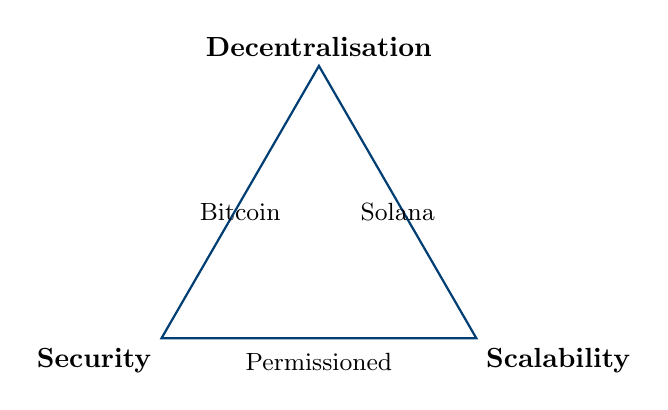
\begin{tikzpicture}[scale=1]
    % Triangle
    \draw[thick, ImperialBlue] (0,0) -- (4,0) -- (2,3.46) -- cycle;
    
    % Labels at vertices
    \node[above] at (2,3.46) {\textbf{Decentralisation}};
    \node[below left] at (0,0) {\textbf{Security}};
    \node[below right] at (4,0) {\textbf{Scalability}};
    
    % Blockchain examples
    \node at (1,1.6) {\small Bitcoin};
    \node at (3,1.6) {\small Solana};
    \node at (2,-0.3) {\small Permissioned};
  \end{tikzpicture}
  \end{center}
  
  \vspace{0.5em}
  This is not a proven theorem---it's an observed engineering trade-off.
\end{frame}

\begin{frame}{Understanding the Trade-offs}
  \textbf{Decentralisation $\longleftrightarrow$ Scalability}
  \begin{itemize}
    \item More nodes = more communication overhead, slower consensus
    \item Bitcoin: ~15,000 nodes, ~7 transactions/second
    \item Visa: Centralised, ~65,000 transactions/second
  \end{itemize}
  
  \vspace{0.5em}
  \textbf{Security $\longleftrightarrow$ Scalability}
  \begin{itemize}
    \item Faster blocks mean less time for propagation, creating more forks and easier attack opportunities
    \item Larger blocks process more transactions but require more storage and bandwidth, pricing out smaller validators
  \end{itemize}
  
  \vspace{0.5em}
  \textbf{Security $\longleftrightarrow$ Decentralisation}
  \begin{itemize}
    \item Stronger security requires more resources (hashpower or stake)
    \item Higher costs push participants toward pools, concentrating power
  \end{itemize}
  
  \vspace{1em}
  Different blockchains make different choices based on their intended use case.
\end{frame}

\begin{frame}{Where Blockchains Sit}
  \begin{center}
  \begin{tabular}{lccc}
    \toprule
    \textbf{Blockchain} & \textbf{Decent.} & \textbf{Security} & \textbf{Scalability} \\
    \midrule
    Bitcoin & \good{High} & \good{High} & \bad{Low ($\approx$7 TPS)} \\
    Ethereum & \good{High} & \good{High} & \bad{Low ($\approx$15 TPS)} \\
    Solana & \bad{Lower} & Medium & \good{High ($\approx$5000 TPS)} \\
    BNB Chain & \bad{Low} & Medium & \good{High} \\
    Hyperledger & \bad{Permissioned} & \good{High} & \good{High} \\
    \bottomrule
  \end{tabular}
  \end{center}
  
  \vspace{1em}
  \textbf{Note}: ``High security'' for permissioned chains means something different---they trust the known validators rather than relying on economic incentives.
  
  \vspace{1em}
  The question is not which is ``best'' but which trade-off suits the application.
\end{frame}

\begin{frame}{Layer 2: Escaping the Trilemma?}
  \textbf{The idea}: Don't do everything on the main chain (Layer 1).
  
  \vspace{1em}
  \begin{block}{Layer 2 Solutions}
    Process transactions off-chain, but inherit security from the main chain by periodically posting proofs or summaries.
  \end{block}
  
  \vspace{0.5em}
  \textbf{Examples}:
  \begin{itemize}
    \item \textbf{Lightning Network} (Bitcoin): Payment channels for instant, low-fee transactions
    \item \textbf{Rollups} (Ethereum): Bundle hundreds of transactions, post compressed data to L1
  \end{itemize}
  
  \vspace{1em}
  Layer 2 doesn't ``solve'' the trilemma---it moves the trade-off. You get scalability but add complexity and different trust assumptions.
\end{frame}

\begin{frame}{Layer 2 in Practice}
  \textbf{Ethereum's scaling roadmap} centres on rollups:
  
  \vspace{0.5em}
  \begin{itemize}
    \item Arbitrum, Optimism (Optimistic Rollups): $\approx$\$10B+ Total Value Locked (TVL) combined
    \item zkSync, StarkNet (ZK-Rollups): Emerging, more complex
    \item Fees: Often 10--100x cheaper than Ethereum mainnet
    \item Speed: Near-instant confirmation, periodic settlement to L1
  \end{itemize}
  
  \vspace{1em}
  \textbf{Bitcoin's Lightning Network}:
  \begin{itemize}
    \item Enables instant Bitcoin payments
    \item Capacity: $\approx$5,000 BTC locked in channels
    \item Adoption: Growing for micropayments, El Salvador's Chivo wallet
  \end{itemize}
  
  \vspace{1em}
  \textbf{Trade-off}: Layer 2 users must trust the rollup operators to some degree, and bridging between L1 and L2 introduces risk. We'll explore DeFi on L2 in Topic 4.
\end{frame}

%----------------------------------------------------------------------------------------
\section{Economic Implications}
%----------------------------------------------------------------------------------------

\begin{frame}{Energy Consumption: The Updated Picture}
  \textbf{Bitcoin} (PoW): estimated $\approx$100--150 TWh/year
  \begin{itemize}
    \item Comparable to countries like Argentina or Norway
    \item Criticism: Environmental impact, carbon footprint
    \item Defence: Increasingly uses renewable/stranded energy; secures \$1T+ network
  \end{itemize}
  
  \vspace{1em}
  \textbf{Ethereum} (post-Merge PoS): $\approx$0.01 TWh/year
  \begin{itemize}
    \item \good{99.95\% reduction} from pre-Merge levels
    \item Comparable to a few thousand households
  \end{itemize}
  
  \vspace{1em}
  
  \textbf{Implication}: Energy criticism now applies specifically to PoW chains (primarily Bitcoin), not blockchain technology generally.
\end{frame}

\begin{frame}{Mining Concentration}
  Despite decentralisation goals, mining tends toward concentration:

\begin{figure}[h]
  \centering
  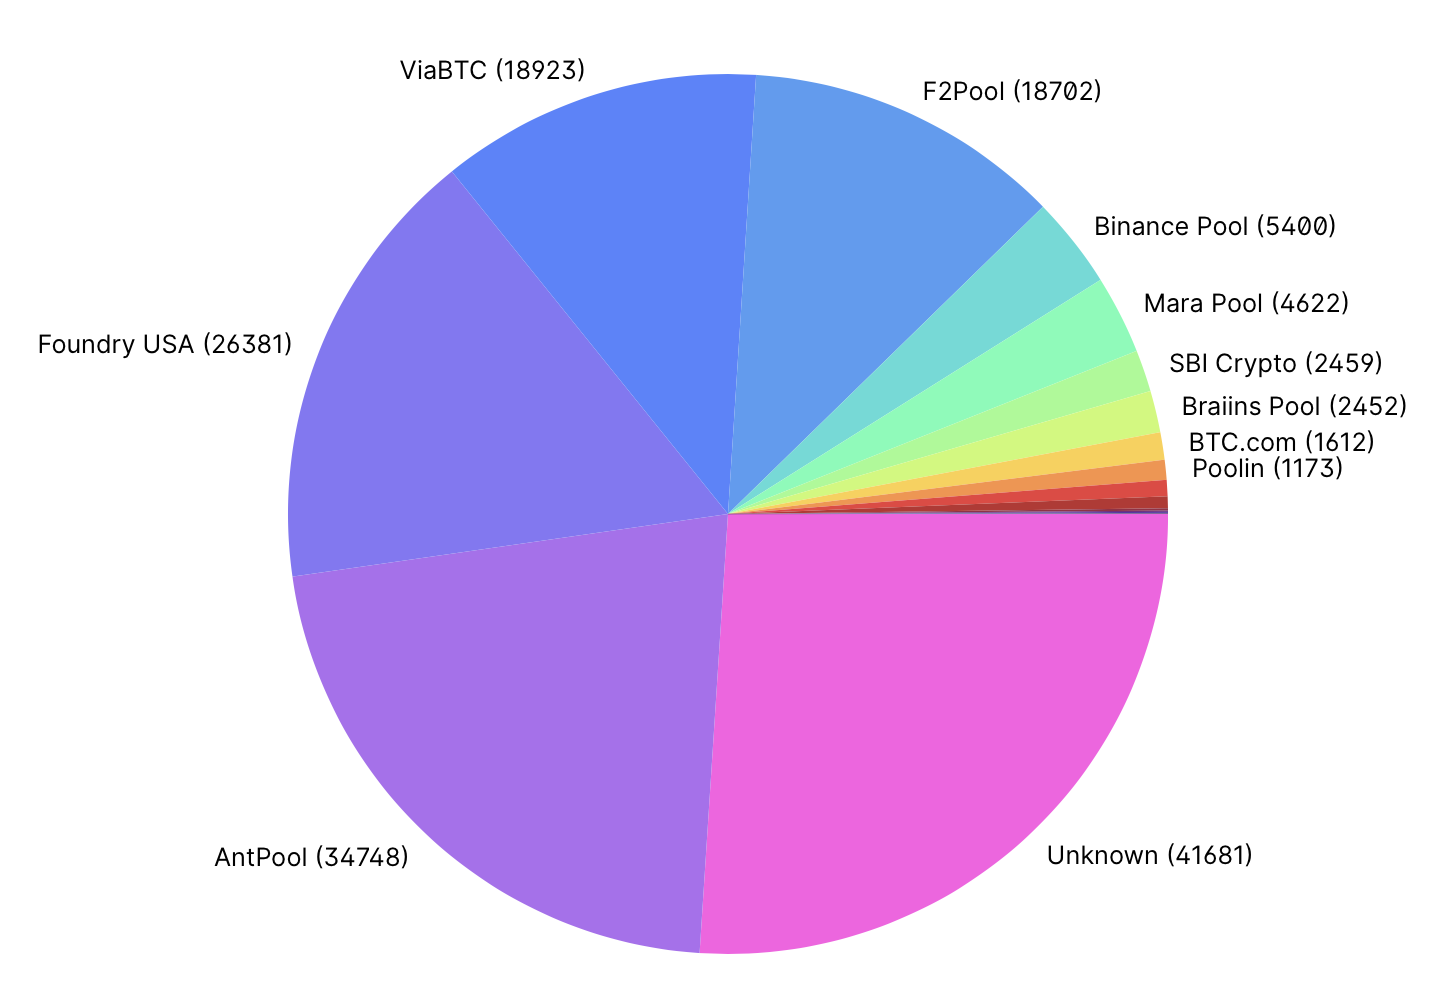
\includegraphics[width=.55\textwidth]{Figures/MiningDistribution Piechart.png}%
  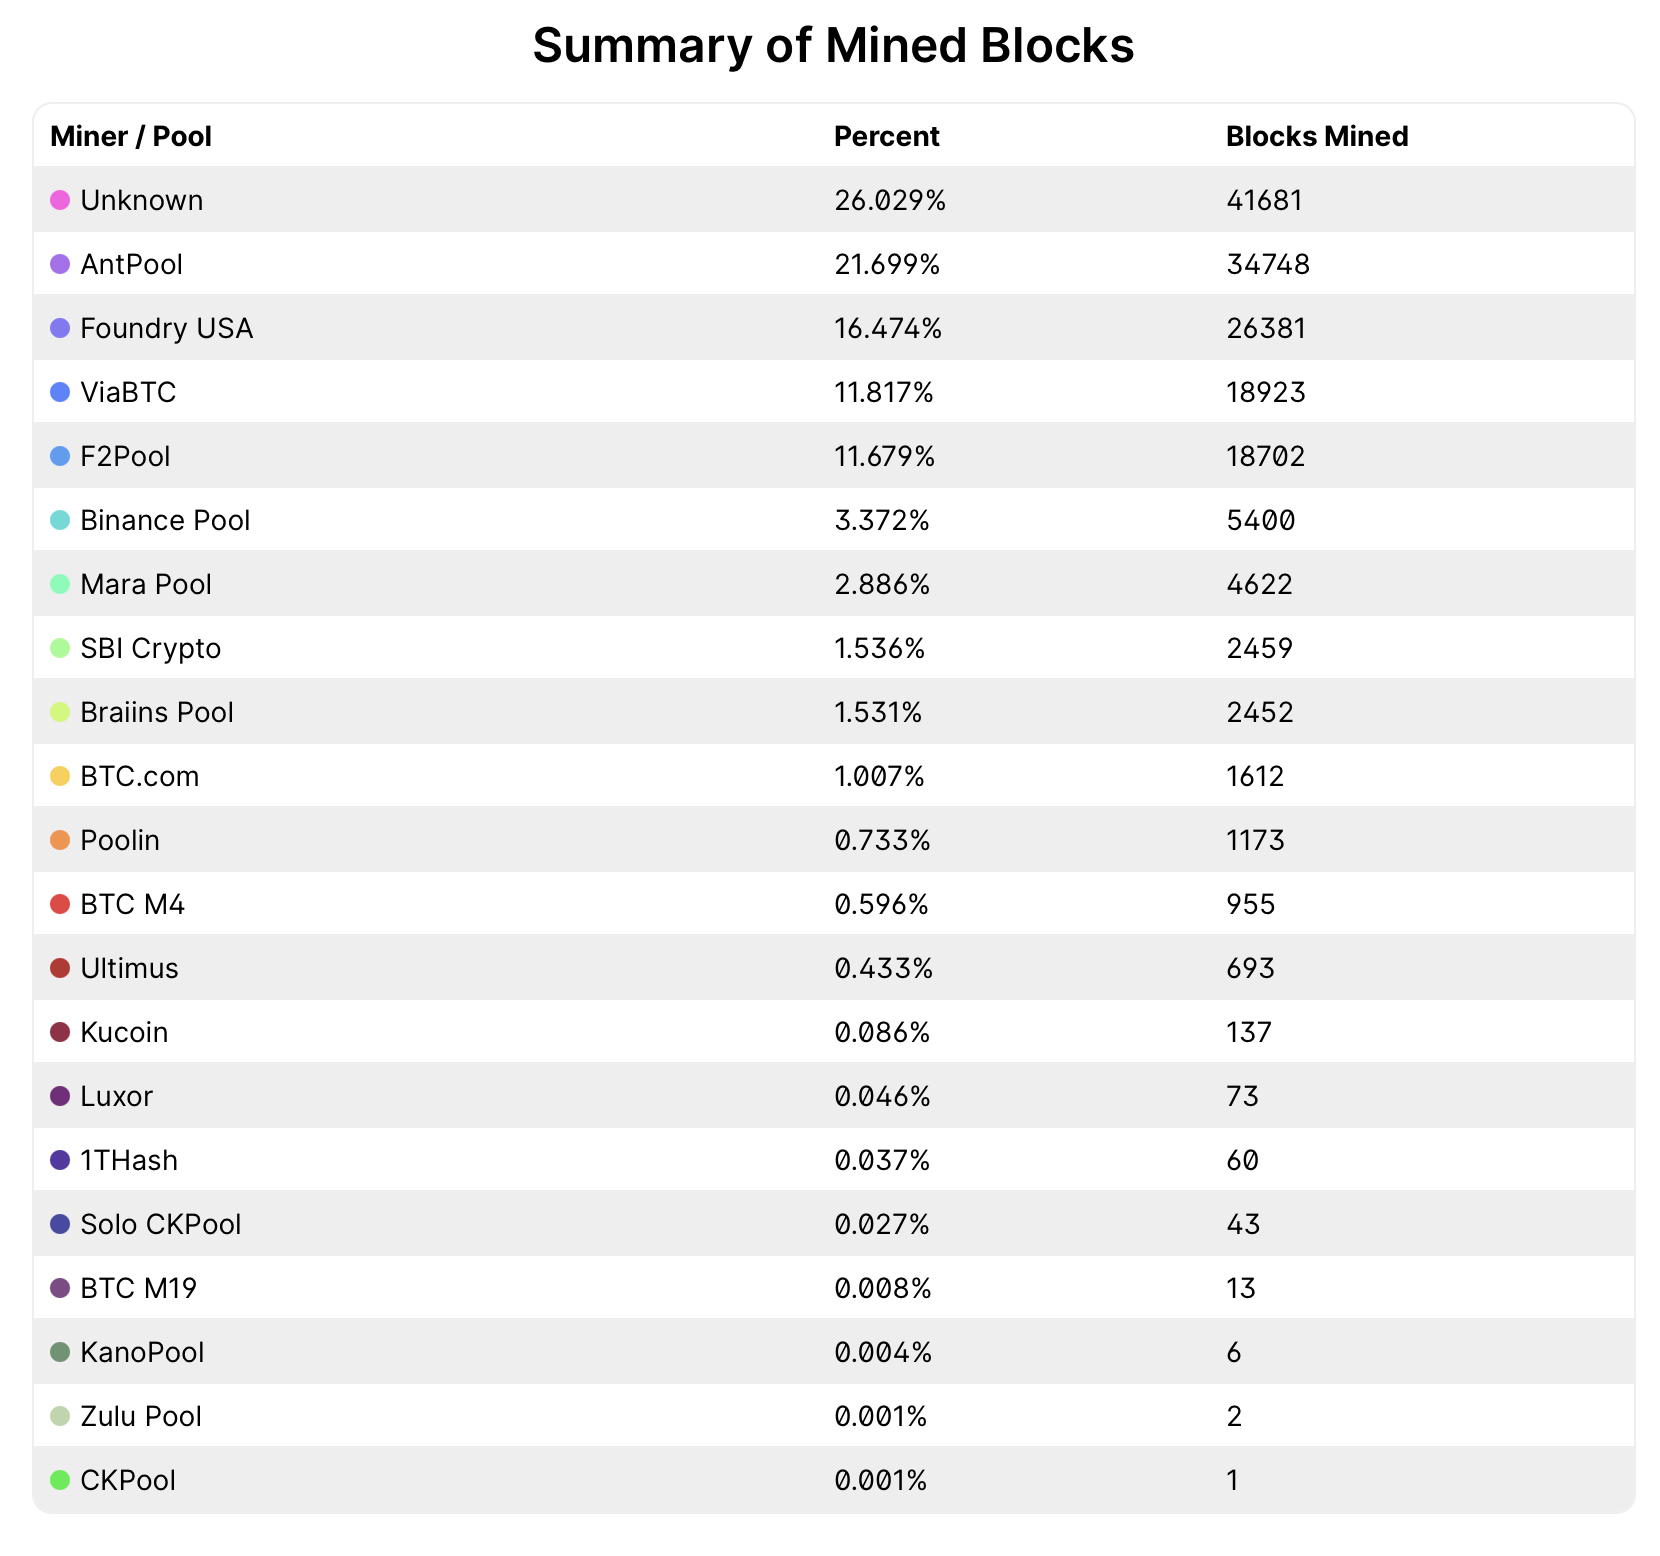
\includegraphics[width=.42\textwidth]{Figures/MiningDistribution Table.png}
\end{figure}

  \textbf{Why concentration occurs}:
  \begin{itemize}
    \item Economies of scale in hardware and electricity
    \item Access to cheap energy sources
  \end{itemize}
  
  \vspace{0.5em}
  \textbf{Nuance}: Pool operators don't control miners' machines. Miners can switch pools, providing some check on pool behaviour.
\end{frame}

\begin{frame}{Wealth Concentration}
  Cryptocurrency holdings are highly concentrated:
  
  \vspace{1em}
  
  \textbf{Bitcoin distribution} (approximate):
  \begin{itemize}
    \item $\approx$70\% of addresses hold less than \$1{,}000 worth of BTC
    \item $\approx$0.01\% of addresses hold more than \$10 million
    \item Concentration is real, but can be misleading: large addresses often represent exchanges, funds, or custodians holding on behalf of many users
  \end{itemize}
  
  \vspace{1em}
  \textbf{Caveats}:
  \begin{itemize}
    \item One person can have many addresses
    \item One address can represent many people (exchanges, funds)
    \item Early adopters naturally hold more (bought at \$1, not \$60,000)
  \end{itemize}
  
  \vspace{1em}
  \textbf{Economic question}: Does this concentration undermine the ``democratising'' narrative? Or is it simply reflecting early-stage adoption patterns?
\end{frame}

\begin{frame}{Staking Concentration}
  PoS introduces similar concentration dynamics:
  
  \vspace{1em}
  \textbf{Ethereum staking} (as of 2024):
  \begin{itemize}
    \item Lido (liquid staking): $\approx$30\% of all staked ETH
    \item Coinbase, Kraken (exchanges): $\approx$15\% combined
    \item Independent validators: minority share
  \end{itemize}
  
  \vspace{1em}
  \textbf{Concern}: If Lido validators collude, they could potentially censor transactions or extract value.
  
  \vspace{1em}
  \textbf{Mitigations}:
  \begin{itemize}
    \item Lido uses multiple independent node operators
    \item Protocol-level discussions on capping any single entity's share
    \item Rocket Pool and others offer more decentralised alternatives
  \end{itemize}
  
  \vspace{1em}
  \textbf{Takeaway}: Decentralisation is a spectrum, not a binary. Both PoW and PoS face concentration pressures.
\end{frame}

\begin{frame}{Scalability and Adoption}
  \textbf{The challenge}: Blockchain throughput vs real-world demand
  
  \vspace{0.5em}
  \begin{center}
  \begin{tabular}{lc}
    \toprule
    \textbf{System} & \textbf{Transactions/second} \\
    \midrule
    Bitcoin & $\approx$7 \\
    Ethereum L1 & $\approx$15 \\
    Solana & $\approx$5,000 (theoretical) \\
    Visa & $\approx$65,000 (peak capacity) \\
    \bottomrule
  \end{tabular}
  \end{center}
  
  \vspace{1em}
  \textbf{When demand exceeds capacity}:
  \begin{itemize}
    \item Fees spike (Bitcoin fees hit \$60+ in congestion)
    \item Users priced out of the network
    \item Adoption stalls for everyday use cases
  \end{itemize}
  
  \vspace{0.5em}
  \textbf{Layer 2 helps}: Arbitrum, Optimism process millions of transactions settling to Ethereum. But bridging complexity remains a barrier.
\end{frame}

%----------------------------------------------------------------------------------------
\section{Summary and Next Steps}
%----------------------------------------------------------------------------------------

\begin{frame}{Key Takeaways}
  \begin{enumerate}
    \item \textbf{Consensus is the core innovation}
    \begin{itemize}
      \item Solves the double-spend problem without trusted third parties
      \item Must be Byzantine fault tolerant
    \end{itemize}
    
    \vspace{0.3em}
    \item \textbf{Proof-of-Work}: Security through computational cost
    \begin{itemize}
      \item Battle-tested (Bitcoin since 2009), but energy-intensive
      \item Halving schedule creates transition to fee-based security
    \end{itemize}
    
    \vspace{0.3em}
    \item \textbf{Proof-of-Stake}: Security through economic stake
    \begin{itemize}
      \item 99.95\% less energy (Ethereum Merge demonstrated this)
      \item Different trust assumptions and centralisation risks
    \end{itemize}
    
    \vspace{0.3em}
    \item \textbf{The trilemma}: Decentralisation, security, scalability---pick two
    \begin{itemize}
      \item Layer 2 solutions shift trade-offs, don't eliminate them
    \end{itemize}
    
    \vspace{0.3em}
    \item \textbf{Concentration is real}: Mining pools, staking pools, wealth
  \end{enumerate}
\end{frame}

\begin{frame}{What's Next}
  \textbf{Topic 3: Smart Contracts and Decentralised Applications}
  \begin{itemize}
    \item What is a smart contract?
    \item Ethereum Virtual Machine (EVM)
    \item DApp architecture and examples
    \item Smart contract security and risks
    \item Gas fees and EIP-1559
  \end{itemize}
  
  \vspace{1em}
  \textbf{Preparation}:
  \begin{itemize}
    \item Think about: What kinds of agreements could be automated if a computer could verify conditions and execute transfers?
    \item Explore: Look at a transaction on Etherscan (etherscan.io)---what information is visible?
  \end{itemize}
\end{frame}

\begin{frame}[plain]
  \vfill
  \begin{center}
    {\Large Questions?}
  \end{center}
  \vfill
\end{frame}

\end{document}